\chapter{Diseño y Ensamblado}
\label{ch:DisenoEnsamblado}

En esta sección se describirán los pasos necesarios para la concreción física
del proyecto.
Se comenzará con la confección e interpretación del diagrama de cañerías e
instrumentación, con el objetivo de validar la solución propuesta en
\ref{sec:SolucionPropuesta}.
Luego se hará énfasis en la construcción de la planta a partir de los elementos
disponibles.
Se describirá en detalle cada uno de ellos y se hará mención de
las decisiones constructivas tomadas durante el ensamblado.

\section{P\&ID}
\label{sec:p&id}

\subsection{Diagrama de cañerías e instrumentación}
Un diagrama de cañerías e instrumentación es un esquema de la planta en donde
pueden observarse todos los elementos que componen el proceso.
Estos diagramas emplean símbolos para representar cada elemento y sus
conexiones.
Los elementos presentes en este esquema están regidos por la norma
\emph{Standard S5.1 Instrumentation Symbol Specification}.

El diagrama permite una rápida comprensión del proceso, y se denomina
corrientemente \gls{pyid}.

En los diagramas \gls{pyid} encontramos graficados los diferentes elementos
como círculos o símbolos representativos, cada uno de ellos acompañado de una
denominación que utiliza la siguiente codificación:

\begin{itemize}  
 \item \textbf{Primer letra:}
 designa la variable medida. Puede ser :
 \begin{itemize}
  \item Presión
  \item Nivel
  \item Caudal
  \item Temperatura
 \end{itemize}

 \item \textbf{Letras siguientes:}
 designa la función del componente, o modifica el sentido de la primer letra.
 Puede ser:
 \begin{itemize}
  \item Indicador
  \item Almacenaje de datos
  \item Controlador
  \item Transmisor
  \item Alarma
 \end{itemize}
\end{itemize}

Así mismo, estos círculos pueden estar intersectados por una línea, la
cual
indica su ubicación:

\begin{itemize}
 \item \textbf{Sin línea:} en el campo.
 \item \textbf{Continua:} en la sala de control.
 \item \textbf{Trazos:} fuera del alcance del operario.
\end{itemize}

Como su nombre lo indica, también están presente en el diagrama la descripción
de las cañerías que forman el sistema (material y diámetros).
Cabe destacar que en esta instancia no es necesario especificar las
longitudes y accesorios.
Esta información forma parte de un diagrama que se debe realizar
en una etapa posterior del proyecto.

También se diferencian en el diagrama la naturaleza de cada señal:

\begin{itemize}
 \item \textbf{Tubería:} línea continua.
 \item \textbf{Señal hidráulica:} línea continua intersectada con líneas
perpendiculares en forma de L.
 \item \textbf{Señal neumática:} linea continua intersectada por pequeñas
líneas paralelas.
 \item \textbf{Señal eléctrica:} línea de trazos.
\end{itemize}

\subsection{P\&ID de nuestra planta}
De acuerdo a los componentes detallados en la Sec.
\ref{sec:MaterialesDisponibles} se realizó el esquema \gls{pyid} de la planta
de control de nivel.
Para la correcta comprensión de este capítulo es indispensable contar con el
esquema, que puede encontrarse en la Fig. \ref{img:pyid}.

\begin{figure}
	\centering
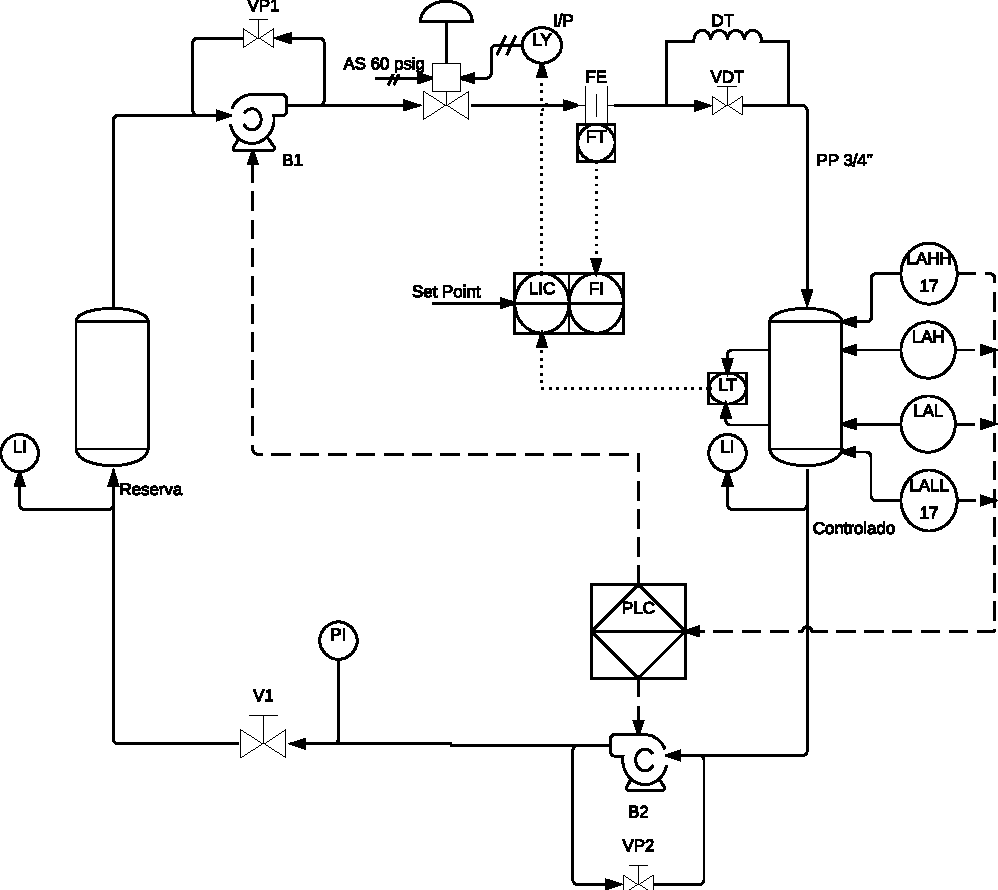
\includegraphics[width=\textwidth]{Cap2-DisenoEnsamblado/images/p&id.pdf}
	\caption{Diagrama P\&ID del proyecto}
	\label{img:pyid}
\end{figure}

Las diferentes partes del diagrama se explicarán a continuación:

\subsubsection{Líneas}

\begin{itemize}
 \item \textbf{Línea de trazos:} $24\,V$.
 \item \textbf{Línea de puntos:} $4$ - $20\,mA$.
 \item \textbf{Línea continua:} tubo de polipropileno de 3/4 pulgada.
\end{itemize}

\subsubsection{Elementos}

En la Tab. \ref{tab:elementos} se presentan los elementos
que forman parte del diagrama \gls{pyid}. Se muestran
los simbolos que tienen cada una de las partes del sistema, así como
también se detalla el significado de las siglas que acompañan a
cada uno.

\begin{table}[H]
\small
\centering
\renewcommand*{\arraystretch}{0.3}

\begin{tabular}{*{2}{m{0.435\textwidth}}}
\hline
Tanque e indicador de nivel en tanque

LI: Level Indicator
  &\begin{center}
    %\rule{0.4\textwidth}{0.3\textwidth}
    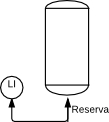
\includegraphics[height = 0.08\textwidth]
	{Cap2-DisenoEnsamblado/images/tanque.png}
  \end{center}\\
\hline
Bomba centrífuga
  &\begin{center}
    %\rule{0.4\textwidth}{0.3\textwidth}
    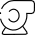
\includegraphics[height = 0.05\textwidth]
	{Cap2-DisenoEnsamblado/images/bomba.png}
  \end{center}\\
\hline
Válvula neumática
  &\begin{center}
    %\rule{0.4\textwidth}{0.3\textwidth}
    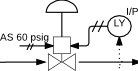
\includegraphics[height = 0.05\textwidth]
	{Cap2-DisenoEnsamblado/images/valvula.png}
  \end{center}\\
\hline
Placa orificio y DP Cell.

FT: Flow Transmitter
  &\begin{center}
    %\rule{0.4\textwidth}{0.3\textwidth}
    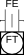
\includegraphics[height = 0.05\textwidth]
	{Cap2-DisenoEnsamblado/images/placa.png}
  \end{center}\\
\hline
Tiempo muerto

DT: Death Time
  &\begin{center}
    %\rule{0.4\textwidth}{0.3\textwidth}
    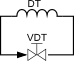
\includegraphics[height = 0.05\textwidth]
	{Cap2-DisenoEnsamblado/images/tmuerto.png}
  \end{center}\\
\hline
Controlador

LIC: Level Indicator and Controller
FI: Flow Indicator
  &\begin{center}
    %\rule{0.4\textwidth}{0.3\textwidth}
    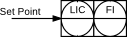
\includegraphics[height = 0.05\textwidth]
	{Cap2-DisenoEnsamblado/images/controlador.png}
  \end{center}\\
\hline
Transmisor e indicador de nivel

LI: Level Indicator
LT: Level Transmitter
  &\begin{center}
    %\rule{0.4\textwidth}{0.3\textwidth}
    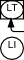
\includegraphics[height = 0.08\textwidth]
	{Cap2-DisenoEnsamblado/images/tnivel.png}
  \end{center}\\
\hline
Válvula e indicador de presión

PI: Pressure Indicator
  &\begin{center}
    %\rule{0.4\textwidth}{0.3\textwidth}
    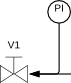
\includegraphics[height = 0.08\textwidth]
	{Cap2-DisenoEnsamblado/images/valvulam.png}
  \end{center}\\
\hline
\hline
\end{tabular}
\caption{Elementos del diagrama P\&ID}
\label{tab:elementos}
\end{table}

\subsubsection{Alarmas} 
\label{subsec:alarmas}

La gestión de alarmas se realiza a través del sensor de nivel presente en la
planta,
tomando la información del mismo para detener el sistema en caso de pasar
los límites normales de trabajo.
Este proceso debería realizarse utilizando sensores separados (redundancia).
No obstante, debido al costo de incluir sensores suplementarios,
se decidió utilizar
directamente el sensor de nivel presente.

En la Tab. \ref{tab:alarmas} se presenta la descripción de cada símbolo de
alarma.

\begin{table}[H]
\small
\centering
\renewcommand*{\arraystretch}{0.3}

\begin{tabular}{*{2}{m{0.435\textwidth}}}
\hline
LAHH: Level Alarm High High
  &\begin{center}
    %\rule{0.4\textwidth}{0.3\textwidth}
    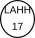
\includegraphics[height = 0.08\textwidth]
	{Cap2-DisenoEnsamblado/images/lahh.png}
  \end{center}\\
\hline
LAH: Level Alarm High
  &\begin{center}
    %\rule{0.4\textwidth}{0.3\textwidth}
    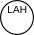
\includegraphics[height = 0.08\textwidth]
	{Cap2-DisenoEnsamblado/images/lah.png}
  \end{center}\\
\hline
LALL: Level Alarm Low Low
  &\begin{center}
    %\rule{0.4\textwidth}{0.3\textwidth}
    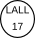
\includegraphics[height = 0.08\textwidth]
	{Cap2-DisenoEnsamblado/images/lall.png}
  \end{center}\\
\hline
LAL: Level Alarm Low
  &\begin{center}
    %\rule{0.4\textwidth}{0.3\textwidth}
    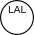
\includegraphics[height = 0.08\textwidth]
	{Cap2-DisenoEnsamblado/images/lal.png}
  \end{center}\\
\hline
PLC: Simbolo de la sección del programador encargado
de la gestión de alarmas
  &\begin{center}
    %\rule{0.4\textwidth}{0.3\textwidth}
    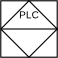
\includegraphics[height = 0.08\textwidth]
	{Cap2-DisenoEnsamblado/images/plc.png}
  \end{center}\\
\hline
\hline
\end{tabular}
\caption{Alarmas en el P\&ID}
\label{tab:alarmas}
\end{table}

\section{Estructura de Soporte}
\label{sec:EstructuraSoporte}

Dado que el objetivo principal del proyecto es que la planta sirva para fines
educativos, se opta por utilizar una estructura móvil.
De esta manera, la posición de la planta puede modificarse según se requiera.

\todo{imagen de la estructura}
La estructura, de caño estructural, puede apreciarse en la figura x.
Está dotada de cuatro ruedas con frenos de seguridad, que permiten fijar la
planta al momento de una demostración.
Sus dimensiones se presentan en la Tab. \ref{tab:dimensionesEstructura}.

\begin{table}
\centering
\begin{tabular}{|l|l|}
\hline
Alto & $1.55\,m$ (incluido ruedas)\\
Ancho &  $1.50\,m$\\
Profundidad &  $0.52\,m$\\
\hline
\end{tabular}
\caption{Dimensiones de la estructura de soporte}
\label{tab:dimensionesEstructura}
\end{table}
 
La estructura presenta en su sección media barras de refuerzo.
Sobre ellas se colocaron los tanques.
Además, sobre las barras se fijó una base de madera, donde se coloca la
válvula electroneumática, las celdas de presión diferencial
y las bombas.
La manguera que corresponde al tiempo muerto se colocó bajo
las barras de refuerzo.
En la parte superior de la planta se instaló una pequeña base de
madera donde irá montado el receptor inalámbrico.
Ya está incluida en la estructura el tablero, donde se
montarán los elementos eléctricos y electrónicos.
Sus dimensiones se observan en la Tab. \ref{tab:dimensionesTablero}.

\begin{table}
\centering
\begin{tabular}{|l|l|}
\hline
Alto & $62\,cm$\\
Ancho &  $30\,cm$\\
Profundidad &  $20\,cm$\\
\hline
\end{tabular}
\caption{Dimensiones del tablero.}
\label{tab:dimensionesTablero}
\end{table}

Al comienzo del proyecto la estructura de caño estaba ya soldada y pintada, con
las ruedas colocadas.
No obstante, el grupo de trabajo tuvo que barnizar las maderas.

\section{Cañerías}
\label{sec:Canerias}

\subsection{Mangueras y Caños}
Luego de analizar el esquema \gls{pyid}, se observa que las cañerías deben
formar un circuito cerrado (\emph{loop}), diferenciando
claramente las cañerías de vaciado y llenado.
Las conexiones fueron echas mayormente en caño de polipropileno de 3/4
pulgadas (presión de servicio: $11.7\,kgf/cm^2$ a $20^\circ C$).
En otros puntos del circuito, se optó por utilizar manguera de alta presión
telada de 3/4 pulgadas (presión de servicio: $10\,kgf/cm^2$ a $20^\circ C$).
Las cañerías utilizadas son suficientes para las presiones de trabajo del
proyecto, del orden de $1.2\,kgf/cm^2$.

Teniendo los elementos montados sobre la planta (bombas, tanques, válvula
electroneumática) se decidió la manera de realizar el conexionado.
El caño rígido presenta la dificultad de no tener tolerancia al momento de
realizar uniones.
Además, para realizar tuberías complejas con muchas curvas, es necesario
colocar un gran número de componentes suplementarios (uniones dobles,
niples).
La cañería se torna compleja, dificultando la comprensión del circuito
hidráulico por parte del alumno.
Es por ello que se opto por usar en diferentes partes de la planta mangueras
flexibles:

\begin{itemize}
  \item \textbf{Salida del tanque de reserva - entrada a la bomba B1}:
  se utilizo manguera flexible dado que la estructura no permitía colocar caños
  rígidos: los elementos de polipropileno necesarios eran más grandes que el
  espacio disponible en la estructura.

  \item \textbf{Salida de la bomba B1 - entrada a la válvula:}
  se utilizo manguera, para evitar una unión doble en un trayecto muy pequeño.
  
  \item \textbf{Salida de la válvula - entrada al tanque controlado:}
  debido a la longitud del tramo se opto usar caños rígidos.
  Además, se montaron los elementos de medición sobre la cañería (manómetro y
  placa orificio).
  
  \item \textbf{Salida del tanque controlado - entrada a la bomba B2:}
  debido al mismo problema de falta de espacio, se opto por el uso de manguera
  flexible.
  
  \item \textbf{Salida de la bomba - entrada al tanque de reserva:}
  esta conexión es la más larga y en ella van montados manómetros y
  válvulas manuales. Por ello, se eligió una cañería rígida de polipropileno.

  \item \textbf{Conexión de perturbación de las bombas:}
  se utilizó manguera flexible, para evitar uniones dobles y
  niples que requieren de una gran precisión durante el montaje.
 \end{itemize}

Por ultimo se procedió a pintar los caños mediante un código de colores.
 \begin{itemize}
  \item {\color{Cerulean} \textbf{Celeste:}} llenado del tanque controlado.
  \item {\color{YellowOrange} \textbf{Amarillo:}} vaciado del tanque controlado.
 \end{itemize}
El código de colores, si bien no es estándar en la industria, permite una fácil
comprensión del circuito hidráulico, (ver Fig. \ref{fig:canerias}.

\begin{figure}[ht]
        \centering
        \begin{subfigure}[b]{0.36\textwidth}
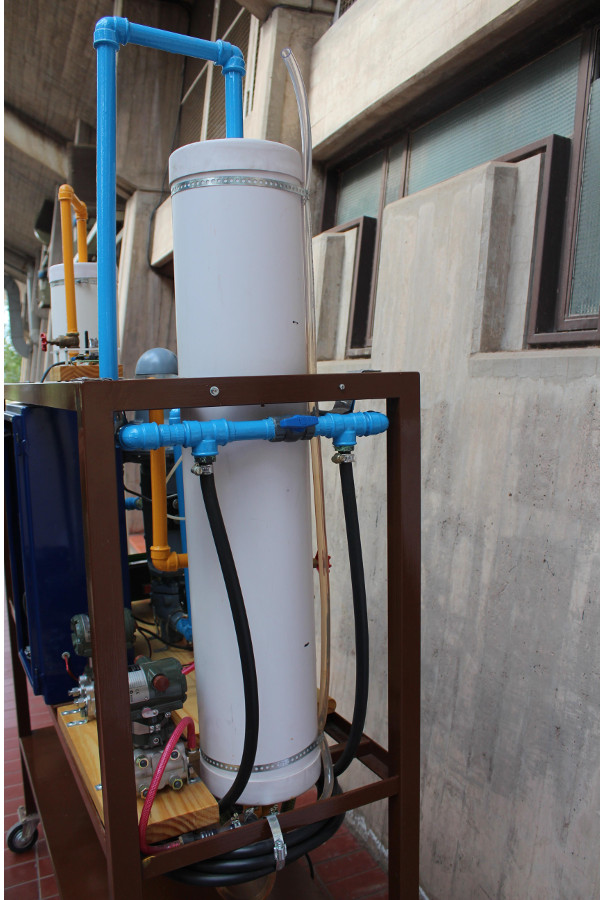
\includegraphics[width=\textwidth]
	{Cap2-DisenoEnsamblado/images/caneria1.JPG}
        \end{subfigure}%
        \hfil
        \begin{subfigure}[b]{0.36\textwidth}
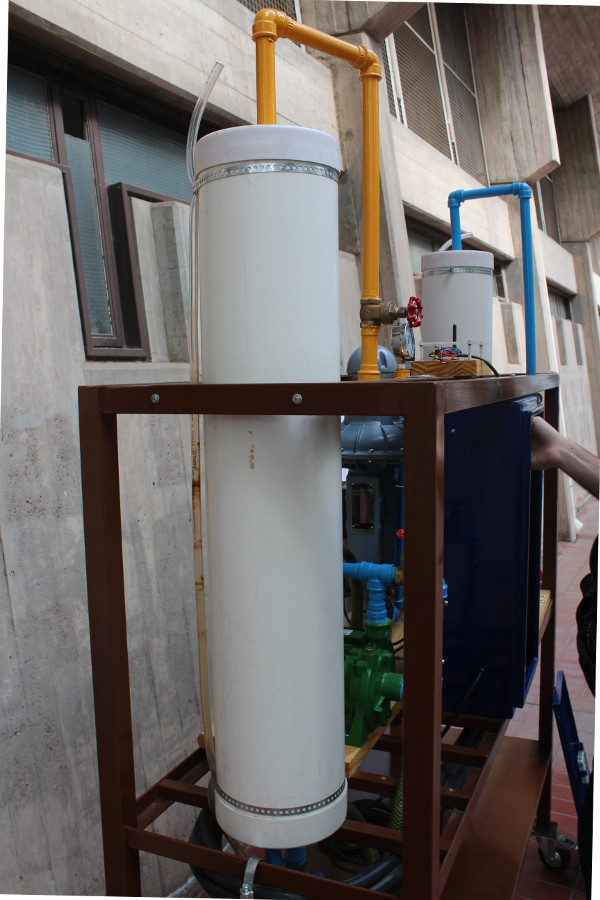
\includegraphics[width=\textwidth]{Cap2-DisenoEnsamblado/images/caneria2.JPG}
        \end{subfigure}
        \caption{Código de colores de las cañerías.}
        \label{fig:canerias}
\end{figure}

\subsection{Tiempo Muerto}
\label{subsec:tiempoMuerto}
Se colocó en la planta un circuito de tiempo muerto, que consta de 20 metros de
manguera negra de 1/2 pulgada.
El tiempo muerto se coloca en paralelo de la cañería de llenado (ver
\gls{pyid}).
Mediante una válvula manual puede elegirse utilizar o no el tiempo muerto.

El objetivo del tiempo muerto es alejar la acción de control del tanque
controlado.
El sensor de nivel tardará un tiempo adicional $t_d$ en observar los cambios
que se producen en la válvula electroneumática \cite{bib:ApuntesPuglesiTema2}.
La función de transferencia de la planta cambiará notablemente:
\begin{itemize}
 \item Por un lado, el retraso en la respuesta debe ser tenido en cuenta
 \begin{align}
  G_{td}(s) &= e^{-t_d\,s}\,G(s)
 \end{align}
 donde $G(s)$ corresponde a la función de transferencia de una planta sin
 tiempo muerto, y $G_{td}(s)$ es la misma planta con tiempo muerto.
  \item Por otro lado, se agregan pérdidas por rozamiento del
  fluido cambiando la función de transferencia original $G(s)$ de nuestra
  planta.
\end{itemize}
En conclusión, el proceso a controlar es diferente comparado con proceso sin
tiempo muerto.
La inclusión esta cañería adicional permite disponer de dos escenarios
diferentes para realizar prácticas, diseñando controladores distintos para
cada caso \cite{bib:ApuntesPuglesiTema2}.

\subsection{Válvulas manuales}

Diferentes válvulas manuales pueden encontrarse en las cañerías de la planta.
A continuación vamos a destacar la función de cada una de ellas:

\begin{itemize}
  \item \textbf{Desagote de los tanques:}
  para poder vaciarlos, se colocaron válvulas esféricas plásticas debajo de
cada tanque.

  \item \textbf{Control de caudal del tanque de reserva:} se colocó en serie
con la cañería de retorno. Se trata de una válvula manual, tipo exclusa.
  Esta válvula es importante ya que permite modificar el balance de masa y
ecualizar la planta.

  \item \textbf{Tiempo muerto:}
  tal como se describió en la Sec. \ref{subsec:tiempoMuerto}, esta válvula
esférica plástica permite activar la cañería de tiempo muerto.
  Notar en el \gls{pyid} que la válvula está sobre la cañería de llenado.
  Al cerrar la válvula, se fuerza el uso del tiempo muerto.
  Al abrirla, nada impide que el fluido circule por las dos cañerías al mismo
tiempo.
  No obstante, la pérdida de carga del tiempo muerto es significativamente
mayor que el de la cañería de llenado.
  Por ello, se considera que al abrir la válvula  el fluido sólo circula
por la cañería de llenado.

  \item \textbf{Perturbación de las bombas:}
  una válvula manual de tipo exclusa se coloca entre la tubería de aspiración y
la tubería de impulsión de las bombas.
  La apertura de esta válvula permitirá simular perturbaciones en las
bombas.
 Al abrir la válvula, el rendimiento de la bomba decae.
 \end{itemize}

\section{Tanques}
\label{sec:Tanques}

Los tanques almacenan el agua que del sistema, y las acciones de
control están dirigidas a establecer el nivel presente en los mismos.
Se ubicaron en los extremos, sobre las barras de refuerzo.
Se fijaron los tanques a las barras laterales de la estructura mediante
abrazaderas.

Son dos caños cloacales de $200\,mm$ de diámetro y un metro de altura, que
fueron
sellados en los extremos utilizando tapas.
La salida de agua hacia la tubería de aspiración de la bomba se realiza
mediante una conexión de tanque de 3/4 pulgada colocada en la base del tanque.
La entrada de agua se realiza por la parte superior, mediante un orificio
sencillo.

Además, en la base del tanque se colocó una segunda conexión de tanque de 3/4
pulgada, que se utilizará para medir el nivel.
Se conectan a esta cañería la celda de presión diferencial y una manguera
flexible transparente.
La manguera flexible, colocada en el lateral del tanque, permite obtener una
lectura visual directa del nivel.
Por otro lado, la celda de presión diferencial es un elemento de adquisición
que permite transformar un valor de presión (altura de la columna de agua) en
una señal $4$-$20\,mA$.
Se discutirá en la Sec. \ref{subsec:DPCell}.

Finalmente, dado que la cañería de aspiración de la bomba puede provocar
perturbaciones en la medición de la celda de presión diferencial, se optó por
colocar un niple en la conexión del tanque de aspiración.
De esta manera, se separan físicamente ambas cañerías, reduciendo las
perturbaciones en la medición de presión.
Cabe destacar que la inclusión del niple limita el nivel mínimo de la planta a
un 15\% del nivel total, aproximadamente.

\section{Bombas}
\label{sec:Bombas}

Se utilizaron en el proyecto dos bombas centrífugas, cuya función es
mantener en movimiento el agua en el sistema.
No se realiza ninguna acción de control sobre las
mismas, por lo que funcionarán de manera continua durante la operación de la
planta.

Las bombas centrífugas son máquinas hidráulicas, que absorben energía mecánica
de un motor y la restituyen en forma de energía hidráulica al fluido.
En las bombas centrífugas (o radiales), esta ganancia de energía se realiza por
medio de la fuerza centrífuga que imparten los álabes del rodete de la bomba.
Este tipo de bomba se caracteriza por entregar una presión elevada y un caudal
relativamente bajo \cite{bib:Mataix}.

Las especificaciones de las bombas utilizadas se presentan en la Tab.
\ref{tab:caractBombas}.

\begin{table}[t]
\centering
\begin{tabular}{|l|l|}
\hline
Marca & Czerweny\\
Caudal máximo &  $100\,l/min$\\
Altura máxima &  $12\,m = 1.2 kgf/cm^2$\\
Tensión & $220\,V$ monofásica $50\,Hz$\\
Corriente & $1.7\,A$\\
Seguridad & S1 IP44\\
\hline
\end{tabular}
\caption{Características de las electrobombas monofásicas}
\label{tab:caractBombas}
\end{table}

\subsection{Cavitación}
\label{subsec:cavitacion}
Para el ingreso del fluido a la bomba, es necesario realizar una succión
en la tubería de aspiración, descendiendo la presión del fluido.
Luego, la presión aumenta violentamente en el rodete de la bomba hasta alcanzar
la altura manométrica.
Debido a la baja presión en la tubería de aspiración, el fluido puede
evaporarse formando burbujas de vapor.
Luego, el rápido aumento de presión provoca una implosión de las burbujas.
Este fenómeno, conocido como \textbf{cavitación} genera ruido y disminuye la
vida útil de las las bombas \cite{bib:ApuntesMDFBombas}.

Para evitar la formación de burbujas de vapor, se opta por mantener la presión
en la tubería de aspiración lo más elevada posible.
Es por ello que las bombas se instalan en una posición baja.
Además, las bombas se colocaron lo más cerca posible de los respectivos
tanques disminuyendo las pérdidas en la cañería de aspiración.
Se fijaron mediante tornillos a la base de madera.

Durante la operación de la planta se observó un correcto funcionamiento de las
bombas, salvo cuando la perturbación se encuentra abierta: al incrementar la
velocidad en la tubería de aspiración, la presión desciende llegando hasta el
punto de vapor.

\section{Válvula Electroneumática}
\label{sec:ValvulaNeumatica}

En esta sección se hará énfasis en la válvula electroneumática.
Es un elemento central en nuestra planta, ya que es la encargada de efectuar
las acciones de control.

\subsection{Principio de funcionamiento}
\label{subsec:principioFuncionamiento}

\begin{figure}[ht]
        \centering
        \begin{subfigure}[b]{0.36\textwidth}
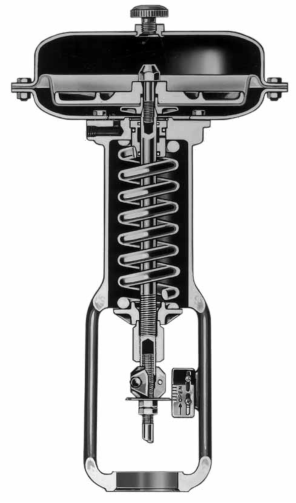
\includegraphics[width=\textwidth]
	{Cap2-DisenoEnsamblado/images/ActuadorValvNeum.pdf}
                \caption{Actuador neumático inverso.}
                \label{fig:actuadorValv}
        \end{subfigure}%
        ~
        \begin{subfigure}[b]{0.36\textwidth}
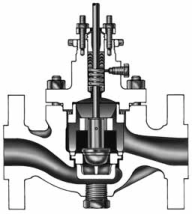
\includegraphics[width=\textwidth]{Cap2-DisenoEnsamblado/images/ValvGlob.pdf}
                \caption{Cuerpo de una válvula globo.}
                \label{fig:cuerpoValv}
        \end{subfigure}
        \caption{Elementos constitutivos de una válvula neumática.}
        \label{fig:elementosValv}
\end{figure}

Una válvula permite variar el caudal, dependiendo de la consigna que se
le envíe.
En las válvulas neumáticas, la consigna es un valor de presión de aire.
En la Fig. \ref{fig:elementosValv} se muestra un ejemplo de válvula de control
tipo globo, con actuador a diafragma inverso (aire para
abrir)\footnote{Figuras extraídas de \cite{bib:controlValveHandbook}.}.
La válvula está compuesta de dos elementos principales: el actuador
(Fig. \ref{fig:actuadorValv}) y el cuerpo de la válvula (Fig.
\ref{fig:cuerpoValv}).

El obturador en el cuerpo de la válvula (Fig. \ref{fig:cuerpoValv}) apoya
sobre un asiento.
La variación del caudal se produce gracias al orificio de paso variable
que forman al variar su posición relativa el conjunto asiento-obturador.
Sobre el vástago, encargado de modificar la posición del obturador,
actúan las fuerzas del actuador.
Como se observa en la Fig. \ref{fig:actuadorValv}, el actuador en una válvula
neumática es el conjunto diafragma-muelle.

Puede concluirse, a través del análisis de la válvula, que el caudal depende de
la presión de aire en el diafragma.
Generalmente, la presión oscila entre $3$ a $15\,psi$.
Esta presión de aire generalmente se obtiene mediante un convertidor
corriente-presión (I/P).
El convertidor toma en entrada una señal de corriente proveniente del \gls{plc}
($4$ - $20\,mA$) y lo transforma en un valor de presión para alimentar el
diafragma \cite{bib:ApuntesPuglesiValvulas}.
% \subsubsection{Rangeabilidad}
% Se denomina rangeabilidad a la razón entre el caudal máximo y el mínimo que
% puede controlar una válvula

\subsubsection{Tipos de obturador - Característica de caudal inherente}
Se denomina característica de caudal inherente a la variación del caudal de
la válvula en función de la carrera, manteniendo una presión diferencial
$\Delta p$ constante.
Para representar la característica inherente de una válvula, se grafica en
abscisas la carrera del obturador y en ordenadas el porcentaje de caudal máximo.

El conjunto asiento-obturador es la parte más importante de la válvula, ya que
es el elemento final que controla el caudal.
Dependiendo del tipo de conjunto asiento-obturador, se obtendrán distintas
características de caudal inherente.
Podemos distinguir tres conjuntos de válvula:
\begin{itemize}
  \item \textbf{Obturador Lineal:} el caudal es proporcional a la carrera
  \begin{align}
	q = k\,l
	\label{eq:inherenteLineal}
  \end{align}
  donde $q$ es el caudal a pérdida de carga constante, $k$ es una constante y
$l$ es la carrera del vástago.

  \item \textbf{Obturador Isoporcentual:}
  un incremento de carrera produce un cambio de caudal proporcional al caudal
que circulaba antes de la variación.
  \begin{align}
    \dfrac{dq}{dl} = a \, q
  \end{align}
  Operando, podemos reescribir esta expresión mediante una función exponencial.
\begin{align}
 q = b\,e^{a\,l}
 \label{eq:InherenteIsoporcentual1}
\end{align}
  donde $a$ y $b$ son constantes para una válvula dada.
  Si consideramos que
    \begin{align}
        l &= 0 \Rightarrow q = q_{min} = b\\
        l &= 1 \Rightarrow q = q_{max} = q_{min} \:e^a
    \end{align}
    podemos escribir la expresión \eqref{eq:InherenteIsoporcentual1} como
    \begin{align}
      \dfrac{q_{max}}{q_{min}} = e^a
    \end{align}
  \item \textbf{Obturador de apertura rápida:} permiten una brusca variación de
caudal con carreras pequeñas.
  No son utilizadas en el control regulatorio, ya que no permiten una
regulación fina del caudal.
\end{itemize}

En la Fig. \ref{fig:caractInherente}, se grafican las curvas de caudal
inherente para cada tipo de válvula.
A simple vista, la válvula con obturador lineal ofrece las mejores
características para el control regulatorio.
No obstante, como se expondrá posteriormente, las curvas características de las
válvulas quedan afectadas por el proceso en el que se utilizan.

\begin{figure}
 \centering
 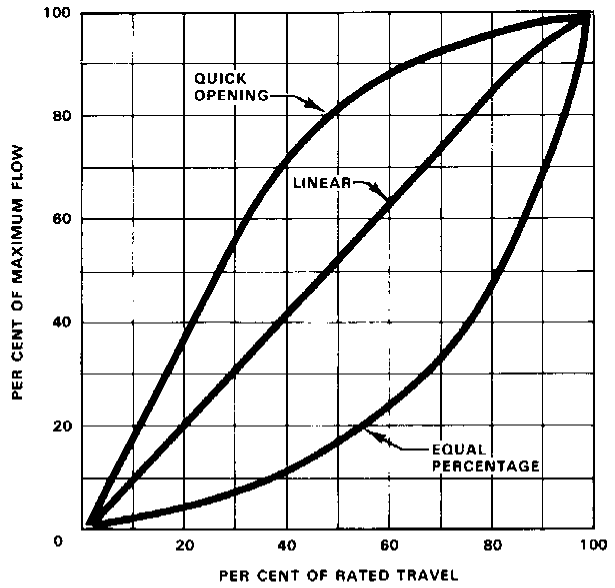
\includegraphics[scale=1.5]{Cap2-DisenoEnsamblado/images/Inherente.png}
 \caption{Características inherentes según el tipo de obturador.}
 \label{fig:caractInherente}
\end{figure}


\subsubsection{Característica de caudal efectivas}

La característica de caudal inherente se traza para una presión diferencial
$\Delta \,p$ constante.
No obstante, en un proceso real, $\Delta \,p$ no es constante.
En efecto, las pérdidas de carga y presión entregada por la bomba presentan
variaciones para diferentes caudales.

Se denomina característica de caudal efectiva a la variación del
caudal que atraviesa la válvula en función de su carrera, cuando la
válvula está inserta en una planta.
Dado que diferentes procesos proporcionarán distintos valores de  $\Delta
\,p$, la característica de caudal efectiva depende del proceso.
Evidentemente, esta curva se apartará de la característica de caudal inherente,
como se demostrará a continuación.

En una cañería, la presión que entregada por la bomba $H$ se utiliza para
vencer las pérdidas de carga en la cañería, contrapresiones y alturas
(reagrupadas en $H_2$) y en la válvula.
Denotando $\Delta \,p = H_1$
\begin{align}
 H &= H_1 + H_2
\end{align}
$H_2$ varía cuadráticamente con el caudal según la ley de \emph{Darcy-Weisbach}
\cite{bib:Franzini}
\begin{align}
 H_2  &= f \dfrac{L}{D^5}\dfrac{16\,Q^2}{2\,g\,\pi^2} + H_c
\end{align}
donde $L$ es la longitud equivalente de la cañería, $D$ es el diámetro y $H_c$
representa la altura piezométrica (contrapresiones y alturas).
$H$ varía siguiendo la curva característica caudal-presión de la bomba.

Se denomina coeficiente $r$ a la razón entre la pérdida de carga de la válvula
$H_1$ comparado con la pérdida de carga total del sistema.
\begin{align}
 r &= \dfrac{H_1}{H_1+H_2} = \dfrac{H_1}{H}
\end{align}
Evidentemente, $r = 1$ cuando la cañería no tiene pérdida de carga,
aproximándose la característica efectiva a la inherente.
Puede demostrarse \cite{bib:Creus} que
\begin{align}
 q_e &= \dfrac{1}{\sqrt{1-r+\dfrac{r}{{q_i}^2}}}
 \label{eq:coef_r_qe_qi}
\end{align}
siendo $q_e$ el caudal efectivo y $q_i$ el caudal inherente, que puede
obtenerse mediante las ecuaciones \eqref{eq:inherenteLineal} y
\eqref{eq:InherenteIsoporcentual1}.

Puede concluirse, a partir de la ecuación \eqref{eq:coef_r_qe_qi} que la curva
de caudal efectivo varía dependiendo de $H_2$.
Si se grafican las características efectivas de diferentes tipos de válvulas,
se observa que al disminuir $r$ (pérdida de carga elevada) una válvula
isoporcentual tiende a comportarse como una lineal,
y una válvula lineal se comporta como de apertura rápida.

Dado que las válvulas de apertura rápida no son utilizadas en el control
regulatorio, se escoge entre una válvula isoporcentual o lineal dependiendo de
la pérdida de carga de la planta, con el objetivo de tener una característica
efectiva ``lo más lineal posible''.

\subsection{Válvula utilizada en el proyecto}

En esta sección se describirá las características específicas de la válvula
utilizada en el proyecto, comparándolas con los principios de funcionamiento
descriptos en la Sec. \ref{subsec:principioFuncionamiento}.

\subsubsection{Especificaciones}
Se muestran en la Tab. \ref{tab:especifValvs} las especificaciones más
importantes de la válvula, consignada en su chapa de identificación.

\begin{table}
\centering
 \begin{tabular}{|c|c|}
  \hline
  Marca & Foxboro\\
  Modelo & V1S-30CNTSSEBK-50\\
	& Stabilflo Serie V1\\
 Actuador & P-50 EA-DO\\
 Medida Cuerpo & 3/4 roscado\\
 Interior & Globo vástago\\
 Característica $C_v$ & $=\%\,CV=10$\\
 Temperatura & $-30$ a $207^\circ C$\\
 Aire para & Abrir  \\
 Carrera & $19\,mm$ \\
  \hline
 \end{tabular}
 \caption{Especificaciones de la válvula electroneumática.}
 \label{tab:especifValvs}
\end{table}

\subsubsection{Electroposicionador}
Se especificó que la presión de aire en el diafragma varía entre $3\,psi$
(válvula cerrada) y $15\,psi$ (válvula abierta).
No obstante, en un convertidor I/P no hay una real comparación entre
la posición del vástago y la señal de corriente.
Ciertos fenómenos como la fricción en el vástago, perturbaciones del fluido,
fuerzas dinámicas, etc. pueden modificar la apertura de la válvula.

Para paliar estos problemas, la válvula incluye un electroposicionador Power
Genex.
Se trata de un controlador proporcional que compara la posición actual del
vástago con la consigna de corriente.
En caso de detectar errores, ejerce la acción de control correctiva para
asegurar la posición del vástago.

\begin{figure}[ht]
 \centering
 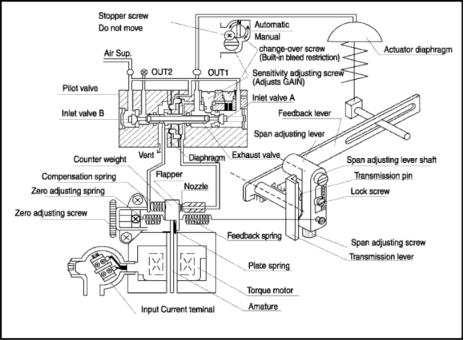
\includegraphics[scale=1.1]{Cap2-DisenoEnsamblado/images/PG-EPL.pdf}
 \caption{Esquema de funcionamiento, posicionador electroneumático.}
 \label{fig:elp-funcionamiento}
\end{figure}

En la Fig. \ref{fig:elp-funcionamiento} se muestra el esquema de
funcionamiento del electroposicionador.
La entrada de $4$-$20\,mA$ del controlador provoca una rotación en sentido
antihorario del motor de torque.
Lleva consigo al \emph{flapper}, liberando
presión por la boquilla (\emph{nozzle}) y moviendo la válvula hacia la
izquierda.
Se provoca un incremento de presión en \emph{OUT1} moviendo el diafragma del
actuador.

La varilla de feedback (\emph{feedback lever}) releva la posición del vástago y
la transmite mediante el resorte de feedback, que está vinculado con el
\emph{flapper}.
Se verifica que la posición del vástago de la válvula permanece constante
cuando el resorte de feedback iguala el par de rotación del motor de torque.
Otros elementos (\emph{compensation spring}, \emph{zero adjusting screw}) se
agregan para poder mejorar la estabilidad del bucle de control, como así
también poder calibrarlo\footnote{Explicación obtenida del manual del
electroposicionador.}.

La Tab. \ref{tab:especifElectroP} muestra las características más importantes
del electroposicionador presente en nuestra planta.

\begin{table}
 \centering
 \begin{tabular}{|c|c|}
  \hline
  Marca & Power Genex\\
  Modelo & EPL-FA15N4TL\\
  Señal entrada & $4$-$20\,mA$ DC\\
  Presión de entrada & $1.4$ - $7\,bar$ máximo\\
  Temperatura de trabajo & $-20$a $70^\circ$\\
  Seguridad & Ex dmb IIB+H2 T6 IP66\\
  \hline
 \end{tabular}
 \caption{Especificaciones del electroposicionador.}
 \label{tab:especifElectroP}
\end{table}

\subsubsection{Característica Efectiva de la válvula}

Como se describió en la Sec. \ref{subsec:principioFuncionamiento}, la
característica de caudal efectiva depende del proceso en donde la válvula esté
inserta.

La característica de caudal efectiva puede encontrarse experimentalmente:
\begin{enumerate}
 \item La planta se coloca en modo manual, encendiendo ambas bombas.
 \item Se coloca la válvula en una posición determinada enviando una consigna
de apertura manual.
 \item Se ecualiza la planta mediante la válvula manual de la cañería de
retorno. Se trata de fijar el nivel de los tanques al 50\%.
 \item Establecido el nivel de la planta (sin oscilaciones) se realiza la
lectura en el DP cell del valor de la presión $h_p$,
y se calcula el caudal correspondiente.
 \item Se cambia la posición de la válvula en intervalos de
 10\%, desde el 0\% (totalmente cerrada) hasta el 100\% (totalmente abierta).
Se repite 3 a 5.
\end{enumerate}

Los resultados se muestran en las Figs. \ref{fig:valvulaStiempoMuerto} y
\ref{fig:valvulaCtiempoMuerto}.
\todo{Sacamos la curva con tiempo muerto?}
En el caso de la planta con tiempo muerto, sólo fue posible realizar mediciones
hasta una carrera del $50\,\%$\footnote{En caso de utilizar carreras mayores,
el manómetro colocado en la cañería de llenado superaba su escala, con el
riesgo consiguiente de rotura.}.

Puede apreciarse un comportamiento aproximadamente lineal de la válvula entre
$10\%$ y $70\%$.
Sobre $70\%$  se produce un fenómeno de saturación conocido como flujo
estrangulado (\emph{choked flow}), que se discutirá posteriormente.
Se concluye que la válvula utilizada es adecuada para el
control regulatorio, debido a su característica efectiva aproximadamente lineal
en la zona de trabajo.

\begin{figure}[ht]
  \centering
  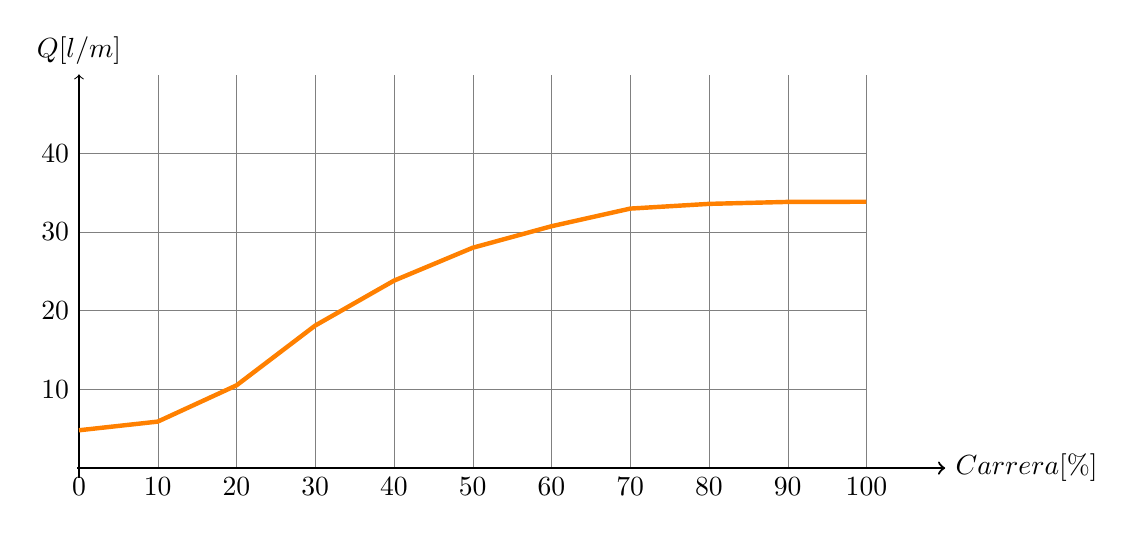
\begin{tikzpicture}[scale= 0.1, domain=0:110]
    
    \draw[ultra thin,color=gray,step=10cm] (100,49.9) grid (0.1,0.1);
    \draw[thick,->] (-0.2,0) -- (110,0) node[right,draw=none] {$Carrera [\%]$};
    \draw[->] (0,-1.2) -- (0,50) node[above,draw=none] {$Q [l/m]$};
    
    \foreach \x in {0,10,20,30,40,50,60,70,80,90,100}
    \draw (\x cm,1pt) -- (\x cm,-1pt) node[anchor=north,draw=none] {$\x$};
    \foreach \y in {10,20,30,40}
    \draw (1pt,\y cm) -- (-1pt,\y cm) node[anchor=east,draw=none] {$\y$};
    
    \draw[color = orange,ultra thick] (0,4.8) -- (10,5.9) -- (20,10.5)
    -- (30,18.1) -- (40,23.8) -- (50,27.98) -- (60,30.71)
    -- (70,32.95) -- (80,33.55) -- (90,33.8) -- (100,33.82);
   
\end{tikzpicture}
\caption{Característica efectiva de la válvula sin tiempo muerto.}
\label{fig:valvulaStiempoMuerto}
\end{figure}

\begin{figure}[ht]
  \centering
  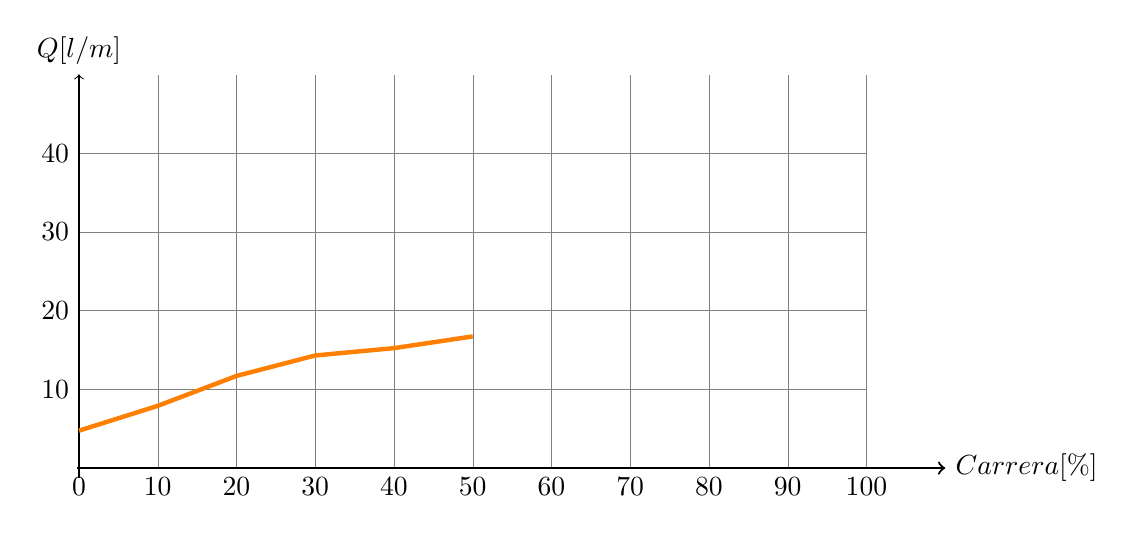
\begin{tikzpicture}[scale= 0.1, domain=0:110]
    
    \draw[ultra thin,color=gray,step=10cm] (100,49.9) grid (0.1,0.1);
    \draw[thick,->] (-0.2,0) -- (110,0) node[right,draw=none] {$Carrera [\%]$};
    \draw[->] (0,-1.2) -- (0,50) node[above,draw=none] {$Q [l/m]$};
    
    \foreach \x in {0,10,20,30,40,50,60,70,80,90,100}
    \draw (\x cm,1pt) -- (\x cm,-1pt) node[anchor=north,draw=none] {$\x$};
    \foreach \y in {10,20,30,40}
    \draw (1pt,\y cm) -- (-1pt,\y cm) node[anchor=east,draw=none] {$\y$};
    
    \draw[color = orange,ultra thick] (0,4.75) -- (10,7.9) -- (20,11.7)
    -- (30,14.3) -- (40,15.23) -- (50,16.72);
   
\end{tikzpicture}
\caption{Característica efectiva de la válvula con tiempo muerto.}
\label{fig:valvulaCtiempoMuerto}
\end{figure}

\subsection{Efecto de flujo estrangulado}
\label{subsec:chokedflow}

Luego de analizar los resultados obtenidos en la pruebas de la planta se pudo
constatar la presencia del efecto de flujo estrangulado o \emph{Choked
Flow}: se observa que la velocidad del fluido permanece constante, a partir de
una carrera del $70\%$.
Posteriores incrementos de la carrera (y por ende, de la presión diferencial
en la válvula) no aumentan la velocidad del fluido en la válvula.

Es una condición dinámica del fluido asociada con el efecto Venturi.
Cuando un flujo de fluido a una presión y temperatura dada pasa a través de una
restricción (por ejemplo: garganta, zona convergente/divergente o válvula),
la presión disminuye y la velocidad del fluido aumenta.
Si la presión desciende por debajo de la presión de vapor, a la
temperatura del fluido se da un fenómeno de evaporación violenta denominado
\emph{flashing}.
Las burbujas entorpecen el paso del líquido, limitando el caudal máximo
\cite{bib:ApuntesPuglesiValvulas}\cite{bib:controlValveHandbook}.

Además, si el fluido regresa a una presión superior a la presión de vapor luego
de pasar por la válvula, se obtiene el fenómeno de cavitación descripto en la
Sec. \ref{subsec:cavitacion}.
La cavitación, además de generar el efecto de flujo estrangulado, produce daños
en el conjunto asiento-obturador.

\subsection{Montaje}
Dada la importancia y tamaño de la válvula, se colocó en el centro de
la planta, sobre la base de madera.
Al momento del montaje se tuvo especial atención en que se pudieran apreciar
con claridad las diferentes partes que la componen.
Se prestó especial atención al nivelado de la válvula.
Finalmente, se fijó mediante ménsulas a la base de madera y a la estructura
de caño.

\section{Instrumentos de Medición}
\label{sec:InstrumentosMedicion}
Para conocer el estado de la planta, es necesario tener conocimiento del
estado de varias variables de la planta, a saber:
\begin{itemize}
 \item \textbf{Nivel de los tanques}
 \item \textbf{Caudal en las tuberías}
 \item \textbf{Presión en las tuberías}
\end{itemize}
Debemos entonces, instalar elementos de instrumentación para poder 
medir y controlar estas variables de interés.

\subsection{DP Cell}
\label{subsec:DPCell}

Se denomina \textit{DP Cell}, o celda de presión diferencial, a un sensor
que mide la diferencia de presión entre dos puntos (ver Fig. \ref{fig:dpcelfig}).
En nuestro caso, la celda entrega una corriente proporcional a la diferencia de
presión medida, en el rango de $4-20\,mA$.
Este valor de corriente será leído por el controlador de la planta.

\begin{figure}[ht]
        \centering
        \begin{subfigure}[b]{0.3\textwidth}
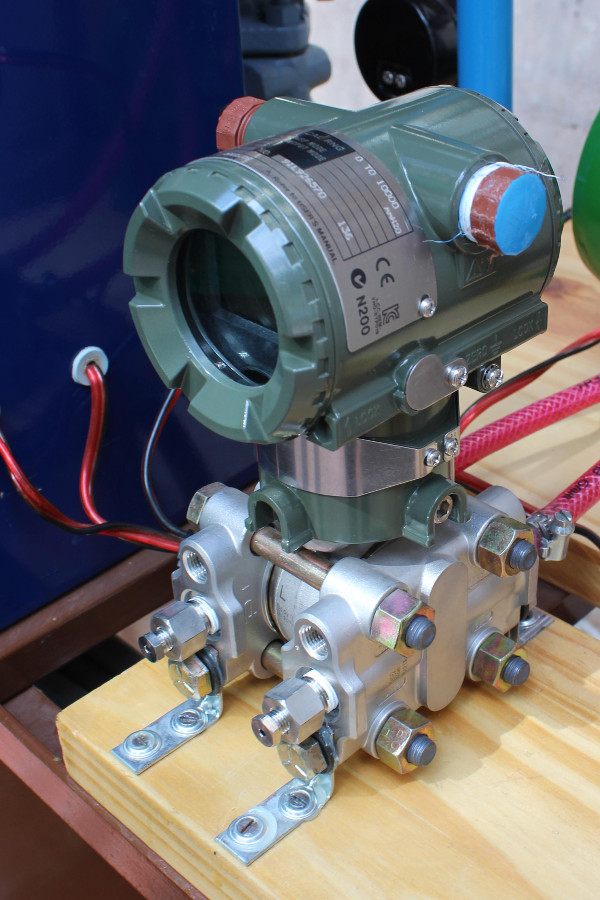
\includegraphics[width=\textwidth]
	{Cap2-DisenoEnsamblado/images/dpcell1.JPG}
        \end{subfigure}%
        \hfil
        \begin{subfigure}[b]{0.6\textwidth}
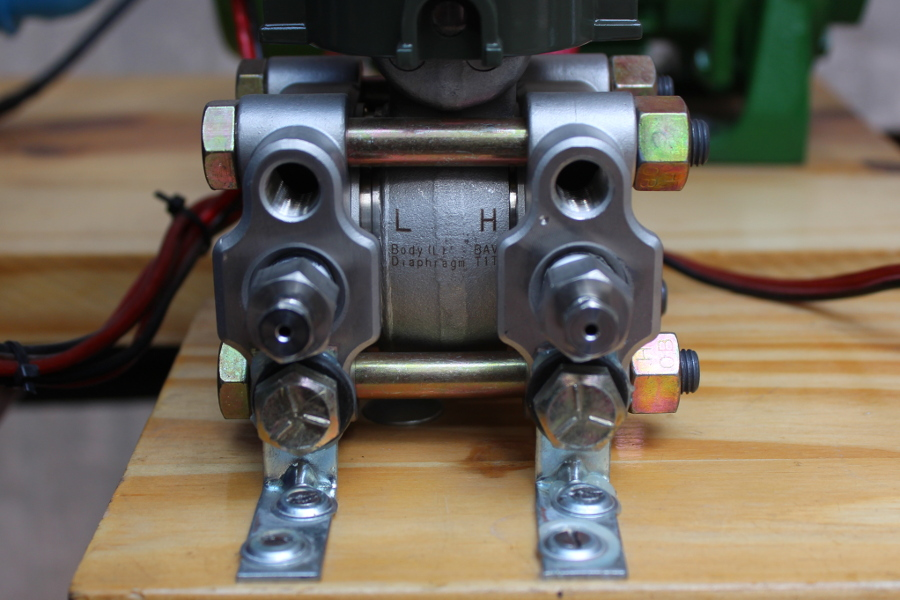
\includegraphics[width=\textwidth]
	{Cap2-DisenoEnsamblado/images/dpcell2.JPG}
        \end{subfigure}
        \caption{DP Cell.}
        \label{fig:dpcelfig}
\end{figure}

Las DP cell utilizadas tienen las especificaciones que se muestran en la Tab.
\ref{tab:caractDPcell}.

\begin{table}
\centering
\begin{tabular}{|l|l|}
\hline
Marca & Yokogawa\\
Modelo & EJA 110 A\\
Sufijo & EMSOA - 22EN / FU1 / D4\\
Tensión & $10.5\,-\,30 \, DC$\\
Output & $4-20\,mA$\\
Presión máxima & $160\,bar$\\
Rango de calibración & $0$ a $10000\,mmCa$\\
\hline
\end{tabular}
\caption{Especificaciones de las celdas de presión diferencial.}
\label{tab:caractDPcell}
\end{table}

Dos celdas serán utilizadas:
\begin{itemize}
 \item \textbf{Medición del nivel del tanque:} una de las entradas de la celda
se conecta  al nivel más bajo del tanque y la otra a presión atmosférica.
La celda mide la presión debida al peso  de la columna de agua en el tanque.
Fue calibrada de manera que entregara un valor de corriente mínimo
cuando el tanque está vacío, y un valor máximo en el caso de que esté
lleno.
Así, el valor entregado por la celda es proporcional al nivel de
agua en el tanque.

\item \textbf{Medición del caudal en la tubería de llenado del tanque
controlado:}
Se utilizará una placa orificio para generar una caída de presión debida al
caudal.
Las entradas de la celda se conectan aguas arriba y aguas abajo
de la placa orificio.
Se mide de esta manera la diferencia de presión entre ambos puntos, que será
traducido en un valor de caudal en el
controlador (ver Sec. \ref{subsec:PlacaOrificio}).
\end{itemize}

Ambas celdas fueron fijadas a la base de madera mediante tornillos.
Las conexiones de las entradas se realizaron con mangueras de alta presión
malladas, de $6\,mm$.

Debemos destacar que, para el caso de la celda de caudal, ambas
entradas se conectaron entre si mediante una válvula manual.
Esta válvula se utiliza solamente durante el primer arranque de la planta:
cuando la cañería está vacía y la bomba B1 se activa, tenemos por una pequeña
fracción de tiempo una presión diferencial de $12\,mCa$ que puede dañar la
celda.
Para evitar este fenómeno, la válvula manual que conecta ambas entradas
permanece abierta durante el primer arranque.
Luego, debe cerrarse para poder realizar la lectura diferencial de presión.

\subsection{Placa Orificio}
\label{subsec:PlacaOrificio}
  se colocó en serie con la cañería de llenado del tanque controlado.
  Debieron instalarse además, las mangueras correspondientes de conexión 
  con la celda de presión diferencial.
  % El tablero se trata en el cap 3 :)
  %\item Tablero electrónico:
  %Estaba montado sobre la estructura una caja estanca donde se montaron todos 
  %los componentes eléctricos
  %y electrónicos.

Para medir el caudal en la tubería de ida, se decide
utilizar una placa orificio\todo{placa orif? u otra cosa?}.
En la Fig. \ref{fig:placaOrificio} se muestra un corte longitudinal de una placa
orificio.
Se observa que la placa orificio provoca una disminución del diámetro
de la cañería, con la consiguiente aceleración del fluido.
Escribiendo la ecuación de Bernoulli en 1 y 2\todo{verif. puntos}.

\begin{figure}
 \centering
 \missingfigure[figwidth=8cm]{Placa orificio}
 \caption{Corte longitudinal de una placa orificio montado en una tubería.}
 \label{fig:placaOrificio}
\end{figure}

\begin{align}
 z_1 \, \gamma + \dfrac{\rho \,v_1^2}{2} + P_1 &= z_2 \, \gamma + \dfrac{\rho \,v_2^2}{2} + P_2
\label{eq:Bernoulli}
\end{align}
donde $z_i$ y $P_i$ es la altura y presión en el punto $i$ y $\rho$ es 
la densidad del fluido. 
Considerando que la altura en ambos puntos es la misma, la ecuación
\eqref{eq:Bernoulli} puede reescribirse como
\begin{align}
 v_2^2 - v_1^2 &= 2\,g\,h_p
 \label{eq:Bernoulli2}
\end{align}
donde $h_p$ es la diferencia de presión entre 1 y 2, expresada como 
altura de la columna fluida
\begin{align}
 h_p &= \dfrac{P_1}{\gamma}-\dfrac{P_2}{\gamma}
\end{align}
La ecuación de continuidad, para fluidos incompresibles se escribe
\begin{align}
 A_1\,v_1 &= A_2\,v_2 \\
 v_2 &= \dfrac{A_1}{A_2} v_1 \\
 v_2 &= \dfrac{D_1^2}{D_2^2} v_1
 \label{eq:velRef}
\end{align}
y reemplazando \eqref{eq:velRef} en \eqref{eq:Bernoulli2} obtenemos
\begin{align}
 2 \, g \, h_p &= v_2^2 \left( 1 - \dfrac{D_1^4}{D_2^4} \right)\\
 \beta &= \dfrac{D_1}{D_2}\\
 v_2 &= \sqrt{\dfrac{2 \, g \, h_p}{1-\beta^4}}
\end{align}
finalmente, el caudal se obtiene multiplicando la velocidad $v_2$ por el
área $A_2$.
Además, se agrega un coeficiente $C_v$ debido al fenómeno de vena contracta:
\begin{align}
 Q &= \dfrac{C_v \, A_2}{\sqrt{1-\beta^4}}\, \sqrt{2 \, g \, h_p}
 \label{eq:placaOrif1}
\end{align}
El coeficiente $C_v$ depende del número de Reynolds $Re$ \cite{bib:Mataix, bib:ApuntesPuglesiPlacaOrif}
\begin{align}
Re &= \dfrac{D\,v}{\nu}
\end{align}
donde $v$ es la velocidad en la placa orificio, $D$ es el diámetro y ${\nu}$
es la viscosidad cinemática del fluido\footnote{Para el agua, nuestro fluido de
trabajo $\nu = 1,003\,10^{-6} \frac{m^2}{s}$.}

La ecuación \eqref{eq:placaOrif1} puede ser reescrita de una forma más sencilla
mediante una nueva variable adimensional $C_q$
\begin{align}
 C_q &= \dfrac{C_v}{\sqrt{1-\beta^4}}
\end{align}
$C_q$, por consiguiente depende tanto del número de Reynolds como de la razón
de los diámetros $\beta$. $C_q$ puede ser encontrado en tablas y ábacos en la
literatura \cite{bib:Mataix}.

No obstante, se observa que el valor de $C_q$ varia poco para valores de
$Re > 20000$, y depende fundamentalmente de $\beta$.
Por ende, puede ser considerado constante para una instalación dada.
Finalmente, la ecuación \eqref{eq:placaOrif1} puede ser expresada como
\begin{align}
 Q &= C_q\,A_2\, \sqrt{2\,g\,h_p}
\end{align}
que puede ser reescrita, teniendo a $C_q$ constante
\begin{align}
 Q &= K\,\sqrt{h_p}
 \label{eq:placaOrifPLC}
\end{align}
donde se observa que el caudal $Q$ es proporcional a la raíz cuadrada de
la diferencia de alturas $\sqrt{h_p}$, que puede
ser encontrada utilizando un DP cell (ver Sec. \ref{subsec:DPCell}).

\subsubsection{Metodología experimental}
Considerando $C_q$ constante,
\begin{align}
 K = C_q\, A_2\, \sqrt{2\,g}
\end{align}
es constante también, y puede ser determinado experimentalmente.
Para ello, se midió sobre el tanque controlado una distancia $l$.
Luego, se encendió la bomba B1 con la válvula electroneumática en posición
abierta (caudal máximo), y se midió el tiempo $t$ necesario para que el nivel
alcanzara la altura $l$.
Ya que el tanque tiene un diámetro $D$, el caudal máximo puede ser
calculado como
\begin{align}
 Q_{max} &= \dfrac{\pi\,D^2\,l}{4\,t}
\end{align}

El módulo analógico del \gls{plc} tiene una resolución de $12\,bits$
(ver Sec. \ref{subsec:plc}), un valor de caudal máximo corresponde a $h_f =
4095$.
$K$ se calcula como
\begin{align}
 K &= \dfrac{Q_{max}}{\sqrt{4095}}
\end{align}
Luego, el caudal puede calcularse fácilmente aplicando la ecuación
\eqref{eq:placaOrifPLC}.

Para la determinación del valor de $K$ se trabajó sin tiempo muerto.
Se marcó en el tanque controlado una altura $l=0.5\,m$, teniendo $D=0.2\,m$.
Luego, se procedió a medir el tiempo de llenado, consignando los resultados en
la Tab. \ref{tab:tiempoK}.

\begin{table}
  \centering
  \bgroup
%   \scriptsize
%   \def\tabcolsep{6.50pt}
%   \def\arraystretch{1.22}%
  \begin{tabular}{|c|c|}
  \hline
  Medición & Valor\\
  \hline
  1 & $27.27\,s$ \\
  2 & $28.53\,s$ \\
  3 & $27.98\,s$ \\
  4 & $28.10\,s$ \\
  5 & $27.68\,s$ \\
  6 & $27.66\,s$ \\
  \hline
  \hline
  \textbf{Media} & $27,87\,s$\\
  \textbf{SD} & $0.43\,s$\\
  \hline
  \end{tabular}
  \egroup
  \caption{Medición del tiempo de llenado, cálculo de $K$.}
  \label{tab:tiempoK}
\end{table}

Finalmente, obtenemos
\begin{align}
 Q_{max} &= 33.81\,\dfrac{lts}{min}
 \\
 K  &= 0.5285\,\dfrac{lts}{min}
\end{align}

\subsection{Manómetros}
\label{subsec:Manometros}

\begin{figure}[ht]
 \centering
 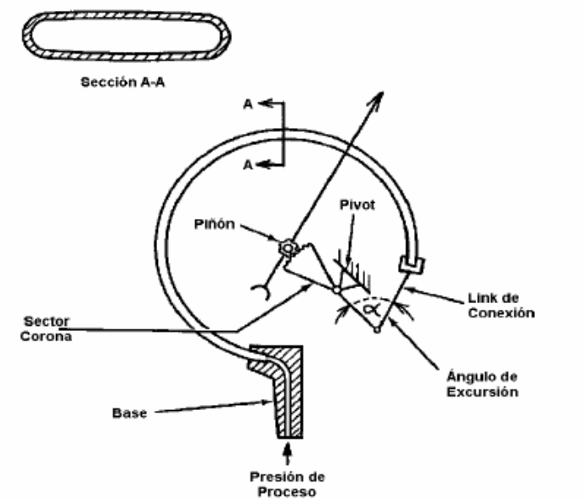
\includegraphics[width=.7\textwidth]{Cap2-DisenoEnsamblado/images/manomBourdon.png}
 \caption{Manómetro de Bourdon, extraído de \cite{bib:ApuntesPuglesiPlacaOrif}}
 \label{fig:manometroBourdon}
\end{figure}

Para conocer los valores de presión en ambas cañerías
(referirse al \gls{pyid}, Sec. \ref{sec:p&id}),
se instalaron manómetros comunes, de tipo Bourdon.
Un ejemplo de estos manómetros se muestra en la Fig. \ref{fig:manometroBourdon}.
Se observa que un incremento de la presión produce una deformación
del \emph{tubo de Bourdon}, reflejado en la aguja indicadora.
El manómetro de Bourdon permite obtener una medición visual de la
presión relativa, del punto donde se encuentra instalado.

Durante el montaje, se presentó el problema que uno de los manómetros
no entregaba una medición definida, sino que oscilaba alrededor de un
valor medio (imposibilitando la lectura directa).
Este problema fue solucionado instalando un \textbf{manómetro con glicerina},
donde el mecanismo del manómetro se encuentra sumergido en un baño de glicerina.
Debido a la viscosidad del fluido, las vibraciones quedan amortiguadas
y el manómetro refleja el valor medio de la presión.

Las especificaciones de los manómetros se muestran en la Tab,
\ref{tab:EspManoms}.

\begin{table}[ht]
\centering
\begin{tabular}{|l|l|}
\hline
Marca & Beyca\\
Rango & $0$ - $1\,kgf/cm^2$\\
 & $0$ - $14\,lb/pulg^2$\\
Escala & $0.02\,kgf/cm^2/div$\\
& $0.5\,lb/pulg^2/div$\\
\hline
\end{tabular}
\caption{Especificaciones de los manómetros}
\label{tab:EspManoms}
\end{table}

En la Fig. \ref{fig:manometro} se observan los dos manómetros 
presentes en el proyecto.
\begin{figure}[ht]
        \centering
        \begin{subfigure}[b]{0.36\textwidth}
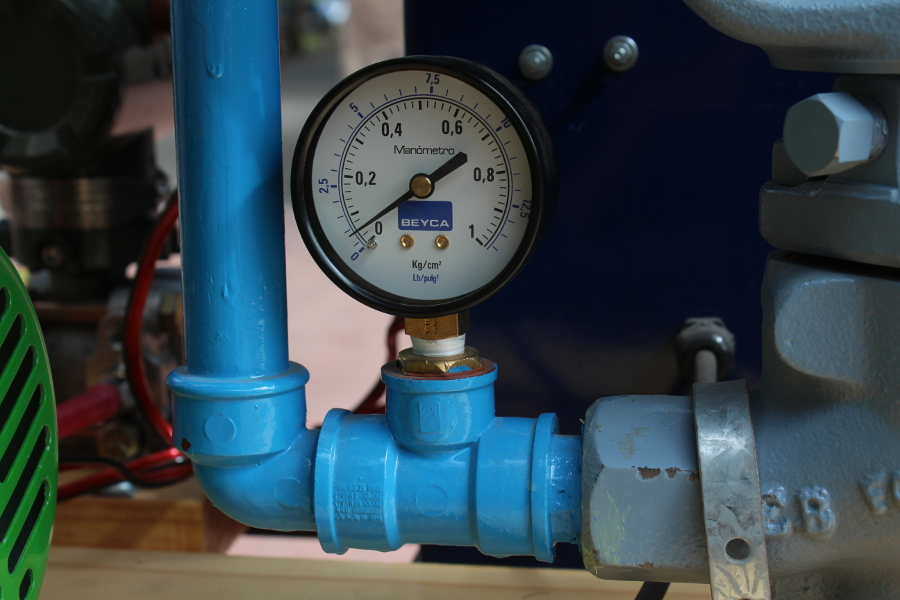
\includegraphics[width=\textwidth]
	{Cap2-DisenoEnsamblado/images/manometro1.JPG}
        \end{subfigure}%
        \hfil
        \begin{subfigure}[b]{0.36\textwidth}
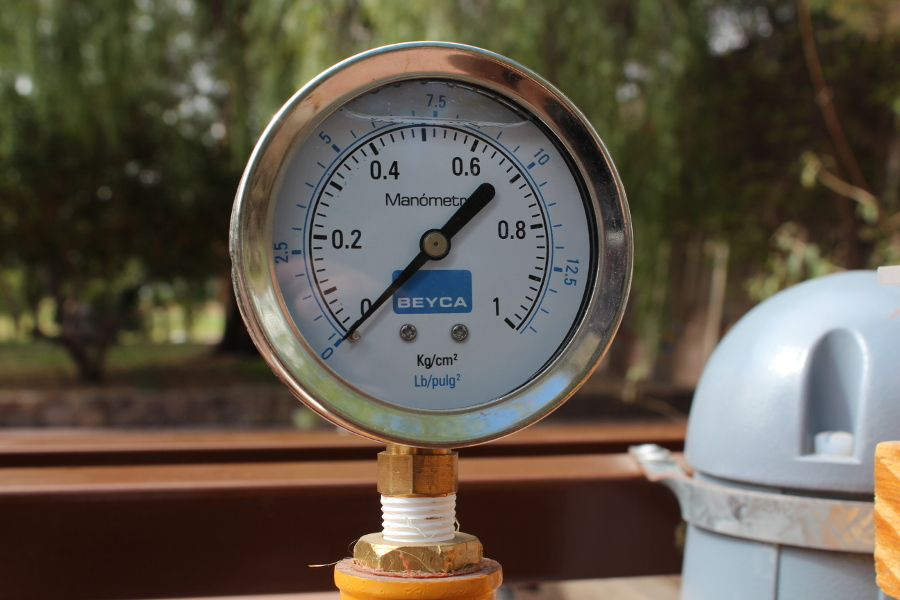
\includegraphics[width=\textwidth]
	{Cap2-DisenoEnsamblado/images/manometro2.JPG}
        \end{subfigure}
        \caption{Manómetros.}
        \label{fig:manometro}
\end{figure}
